% Created 2017-02-28 Tue 09:24
% Intended LaTeX compiler: pdflatex
\documentclass[a4paper,11pt,DIV=18]{scrartcl}
                \usepackage{array}
                \usepackage[utf8]{inputenc}                   
                \usepackage[T1]{fontenc}
                \usepackage{lmodern}
                \usepackage[normalem]{ulem}
                \usepackage{booktabs}
                \usepackage{amsmath,amssymb,amsthm}
                \PassOptionsToPackage{hyphens}{url}
                \usepackage{hyperref}\hypersetup{colorlinks=true,hypertexnames=false}
                \usepackage[osf,sc]{mathpazo}
                \usepackage{booktabs}
                \usepackage{graphicx}
                \usepackage{csquotes}
                \usepackage[usenames,dvipsnames]{xcolor}\definecolor{bg}{rgb}{0.95,0.95,0.95}
                \usepackage[english]{babel}\usepackage{minted}\usemintedstyle{emacs}
\usepackage{tikz}\usepackage{pgfplots}\usepgfplotslibrary{dateplot}\usetikzlibrary{shapes,arrows}\usepackage[]{tcolorbox}
\newtcolorbox[auto counter,number within=section]{work}[1][]{colback=black!5!white,colframe=black!50!white,fonttitle=\sffamily\bfseries,title=Work~\thetcbcounter: #1}
\author{Mathieu Fauvel}
\date{\today}
\title{Labwork Remote Sensing\\\medskip
\large How to use and to extract information from remote sensing images for land management ?}
\begin{document}

\maketitle
\setcounter{tocdepth}{2}
\tableofcontents

\section{Introduction}
\label{sec:org49f0a9b}
\subsection{Objectives of the labworks}
\label{sec:org948310c}
The main objective of these labworks is to
\begin{center}
\emph{be able to  use and to extract information from  remote sensing images
for land management}.
\end{center}
Information  can be  any knowledge  of a  given landscape  (landcover,
land-use, humidity, \ldots{})  that is used to understand the configuration
and/or the evolution of landscape.

In terms of  \emph{competences}, you should be  able to master at  the end of
the sessions  the items listed in  tables \ref{tab:org3564b28}, \ref{tab:org72cedb8}, \ref{tab:org56822c9},  \ref{tab:orgc74e842} and \ref{tab:org1774764}.
Each of them  is organized as a  set of tasks that  should be mastered
progressively.

\begin{table}[htbp]
\caption{\label{tab:org3564b28}
Choose images with properties adapted to your problematic.}
\centering
\begin{tabular}{lp{0.85\linewidth}}
\toprule
\emph{Remember} & Properties of remote sensing images.\\
\emph{Understand} & Physical meaning of each sampling of a given image.\\
\emph{Apply} & Open and visualize a remote sensing image, extract its properties.\\
\emph{Analyze} & Describe a remote sensing image. Recognize specific object.\\
\emph{Evaluate} & Choose the good image adapted to what you are looking for.\\
\emph{Create} & Create a set of properties needed for your problematic.\\
\bottomrule
\end{tabular}
\end{table}

\begin{table}[htbp]
\caption{\label{tab:org72cedb8}
Compute and use spectral indices.}
\centering
\begin{tabular}{lp{0.85\linewidth}}
\toprule
\emph{Remember} & Definition of spectral indices in general and of the NDVI in particular.\\
\emph{Understand} & What (and why) does the NDVI emphasize.\\
\emph{Apply} & Perform the computation of spectral indices.\\
\emph{Analyze} & Analysis of the vegetation cover using NDVI.\\
\emph{Evaluate} & Choose the right spectral index.\\
\emph{Create} & Select from the literature a set of possible indices.\\
\bottomrule
\end{tabular}
\end{table}

\begin{table}[htbp]
\caption{\label{tab:org56822c9}
Define, identify and analyze radiometric behavior.}
\centering
\begin{tabular}{lp{0.85\linewidth}}
\toprule
\emph{Remember} & Spectral signature for \emph{vegetation} and \emph{water} object.\\
\emph{Understand} & Histogram of images.\\
\emph{Apply} & Compute an histogram.\\
\emph{Analyze} & Extract radiometric properties of some classes.\\
\emph{Evaluate} & Choose relevant  spectral  bands and/or  indices for  the  segmentation of several classes.\\
\emph{Create} & Perform a segmentation using radiometric statistics on one or many spectral variables and/or indices.\\
\bottomrule
\end{tabular}
\end{table}

\begin{table}[htbp]
\caption{\label{tab:orgc74e842}
Do and analyze pixel-wise classification of image}
\centering
\begin{tabular}{lp{0.85\linewidth}}
\toprule
\emph{Remember} & Definition of pixel-wise supervised classification.\\
\emph{Understand} & The parameters of  several classification algorithm, how  the spatial sampling of the ground truth data influence the training  and validation steps.\\
\emph{Apply} & Classification algorithms.\\
\emph{Analyze} & Interpret the confusion matrix and the thematic map, the  quality of a ground truth.\\
\emph{Evaluate} & Compare two classification maps/results.\\
\emph{Create} & Choose the most appropriate classifier for one given  application, build good ground truth data.\\
\bottomrule
\end{tabular}
\end{table}

\begin{table}[htbp]
\caption{\label{tab:org1774764}
Define and implement a processing chain}
\centering
\begin{tabular}{lp{0.85\linewidth}}
\toprule
\emph{Remember} & How to  combine several bands, apply a given  function to train  a classifier or to predict a thematic map.\\
\emph{Understand} & The different  inputs and outputs of  \texttt{OTB} functions, how  to use their corresponding documentation.\\
\emph{Apply} & Apply a set of different functions in a pipeline.\\
\emph{Analyze} & Define the different processing needed to perform a given task.\\
\emph{Evaluate} & Evaluate the accuracy of the given processing, check for errors.\\
\emph{Create} & Shell scripts that automatize most the processes, in order to  apply them  on a large set of images  or to apply  several embedded  processes.\\
\bottomrule
\end{tabular}
\end{table}

\subsection{Remote sensing software}
\label{sec:org0ba5430}
In these  labworks, \href{https://www.fsf.org/}{free and  open sources  softwares} will be  used to
visualize  remote sensing  images, to  process them  and to  implement
processing  chains.  In  the  following, each  software/tools will  be
briefly described.  Interested reader can find more information on the
associated website.   In particular,  the installation process  is not
detailed. However, they  can be freely download and  installed on many
operating systems from their official website.

\subsubsection{Orfeo ToolBox (OTB)}
\label{sec:org9f641a8}
\href{https://www.orfeo-toolbox.org/}{OTB} is a C++ library for remote sensing images processing. It has been
developed by the  \href{https://cnes.fr/en}{CNES} (French space agency) during  the ORFEO program
to \emph{prepare, accompany and promote the use and the exploitation of the
images derived from \href{https://en.wikipedia.org/wiki/Pleiades\_\%28satellite\%29}{Pleiades satellites} (PHR)}.  Processing tools from
OTB  are appropriated  to big  images.  When  possible, processes  are
paralyzed and tiled automatically for users. Many applications derived
from OTB and  called \emph{OTB-Applications} are directly usable  for most of
the common processing, they are described \href{https://www.orfeo-toolbox.org/CookBook/CookBook.html}{here}. For advanced users, it
is  possible  to  develop  program  based  on  the  OTB  library  (not
considered in these labworks).

\emph{Monteverdi2} is \emph{graphical user interface} that allows users to visualize
and process  remote sensing images  with \emph{OTB-Applications}. It  is also
developed by the CNES during the ORFEO program. 

\subsubsection{QGIS}
\label{sec:orgaa9b68a}
\href{http://www.qgis.org/en/site/}{QGIS} is  a \emph{Geographic Information System}  (GIS).  It is used  to open,
visualize  and  process  digital  map.  It  includes  several  spatial
analysis tools working mainly on vector  data. QGIS can be extended by
several plugin  (\url{https://plugins.qgis.org/}) and  modules, such  as the
OTB applications.

\subsubsection{Geospatial Data Abstraction Library (GDAL)}
\label{sec:orgb68f7b8}
\href{http://www.gdal.org/}{GDAL}  is   a  library  for   the  processing  of  raster   and  vector
data. Similar  to OTB, it  has several  applications that can  be used
directly. For advanced users, it  is possible to develop program based
on the GDAL library (not considered in these labworks).

\subsubsection{Python}
\label{sec:org48d380a}
\href{https://www.python.org/}{Pyhton}  is   a  programming  language.  It   has  several  programming
capabilities, such as \emph{object-oriented}, \emph{functional programming}, \emph{dynamic
type}  and  \emph{memory management}  that  make  it  widely used  in  several
applications:
\begin{itemize}
\item Web and internet development,
\item Scientific and numeric computing,
\item Software development.
\end{itemize}
It has a large  number of available packages that can  be used in many
applications. For instance, it is possible to call \emph{OTB-Applications} or
\emph{GDAL} from Python.
\subsection{Sequences}
\label{sec:orgc9c1c1c}
\begin{table}[htbp]
\caption{Sequences}
\centering
\begin{tabular}{llrl}
\toprule
Séquences & Type & Volume & Séance\\
\midrule
\textit{<2017-02-28 Tue 10:10>--<2017-02-28 Tue 12:10>} & CTD & 02:00:00 & Visualization of remote sensing data\\
\textit{<2017-02-28 Tue 13:30>--<2017-02-28 Tue 17:30>} & CTD & 04:00:00 & Spectral indices + Segmentation of remote sensing images\\
\textit{<2017-02-02 Thu 10:10>--<2017-02-02 Thu 12:10>} & CTD & 02:00:00 & Detection of floods\\
\textit{<2017-03-08 Wed 13:30>--<2017-03-08 Wed 17:00>} & CTD & 04:00:00 & Classification of remote sensing images\\
\textit{<2017-03-10 Fri 13:30>--<2017-03-10 Fri 15:30>} & CTD & 00:00:00 & \textbf{Non présentiel} -> Spatial distribution of pixels\\
\textit{<2017-03-10 Fri 15:30>--<2017-03-10 Fri 17:30>} & CTD & 02:00:00 & SITS 1/2\\
\textit{<2017-03-14 Tue 10:10>--<2017-03-14 Tue 12:10>} & CTD & 02:00:00 & SITS 2/2\\
\textit{<2017-03-14 Tue 13:30>--<2017-03-14 Tue 15:30>} & CTD & 00:00:00 & \textbf{Non présentiel} -> Best couples of dates\\
\textit{<2017-03-14 Tue 15:30>--<2017-03-14 Tue 17:30>} & CTD & 02:00:00 & Dynamic Habitat Index 1/2\\
\textit{<2017-03-16 Thu 10:10>--<2017-03-16 Thu 12:10>} & CTD & 02:00:00 & Dynamic Habitat Index 2/2 + reviews\\
\textit{<2017-03-23 Thu 10:10>--<2017-03-23 Thu 12:10>} & CTD & 02:00:00 & EXAM Groupe 1\\
\textit{<2017-03-24 Fri 10:10>--<2017-03-24 Fri 12:10>} & CTD & 02:00:00 & EXAM Groupe 2\\
\midrule
Total &  & 30:00:00 & \\
\bottomrule
\end{tabular}
\end{table}

\subsection{During the labworks}
\label{sec:org4b32649}
For the \emph{presential} sequences, you won't have to do any report. But you
will have to  write your personal material on remote  sensing. You are
encouraged to write it progressively  during the sessions.  \textbf{It will be
the only  document approved for the  exam} (with those on  moodle). The
length  of each  sequence  should let  you enough  time  to write  the
report.

For  the \emph{non  presential}  sequences,  you will  be  asked  to write  a
document  that  describe briefly  the  results  and how  you  obtained
them.  Discussion between  all groups  will  be done  during the  next
session.
\section{Data sets}
\label{sec:org74690f6}
\subsection{Pleiades images}
\label{sec:org06fd96d}
These images were acquired over the  Fabas forest in 2013. Images were
acquired   the   \textit{<2013-10-12 Sat>    }    and   the   \textit{<2013-12-10 Tue>},
respectively. A true color composition is given in Figure \ref{fig:org2d526b1}.

\begin{figure}[htbp]
\centering
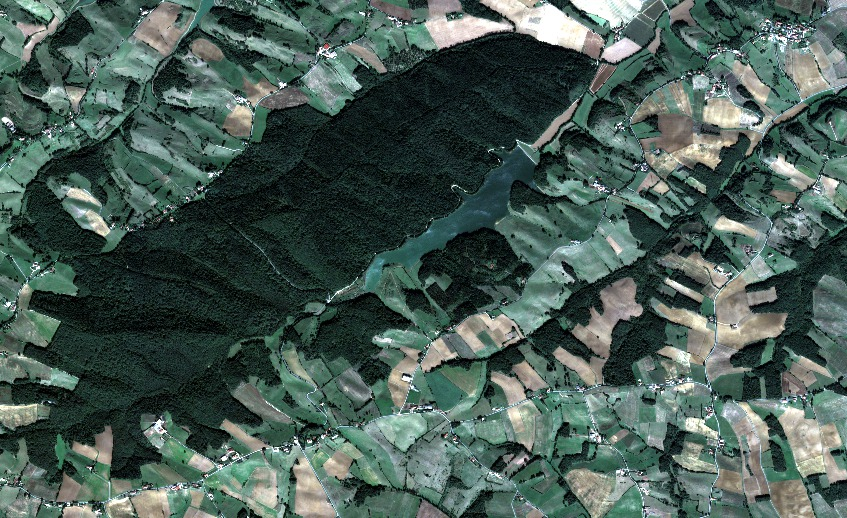
\includegraphics[width=0.5\textwidth]{./figures/quicklook_fabas_12_10_2013.jpg}
\caption{\label{fig:org2d526b1}
Fabas image acquired the \textit{[2013-10-12 Sat]}.}
\end{figure}

Images are stored using the \href{https://trac.osgeo.org/geotiff/}{GeoTIFF} format.  It is an extended version
of  the TIFF  format,  which allows  to  embed geospatial  information
within the file. GeoTIFF can be read by most of the remote sensing and
GIS software. Table \ref{tab:org70d3c22} gives the band order of the data.

\begin{table}[htbp]
\caption{\label{tab:org70d3c22}
Bands and channels information for the Pleiades images}
\centering
\begin{tabular}{rl}
\toprule
Band & Channel\\
\midrule
1 & Red\\
2 & Green\\
3 & Blue\\
4 & Infra-red\\
\bottomrule
\end{tabular}
\end{table}

\subsection{Formosat 2 Satellite image time series}
\label{sec:orgdbb25a6}
\begin{figure}[htbp]
\centering
\includegraphics[width=0.5\textwidth]{figures/sits_f2.png}
\caption{\label{fig:orgf99d25a}
Formosat 2 image acquired the \textit{[2012-05-03 Thu]}.}
\end{figure}

This time series was acquired in 2012 over the region of \emph{Saint Lys}. It
consists  in  a  set  of   \href{http://www.satimagingcorp.com/satellite-sensors/other-satellite-sensors/formosat-2/}{Formosat-2}  images  along  the  year  2012.
Figure~\ref{fig:SITS} provide information  about the acquisition
date and the Figure~\ref{fig:orgf99d25a} shows a false colors composition for
the date \textit{[2012-05-03 Thu]}.

\begin{figure}[tb]
  \centering
  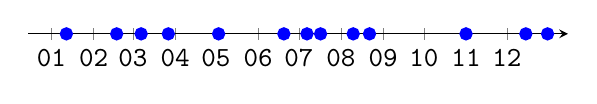
\begin{tikzpicture}
    \begin{axis}[hide y axis,axis lines=middle,
      date coordinates in=x,
      xticklabel={\texttt{\month}},
      x tick label style={},
      date ZERO=2011-12-12,
      xmin=2011-12-15, 
      xmax=2013-01-15,
      ymin=-0.25,ymax=0.25,
      xtick={{2012-01-01},{2012-02-01},{2012-03-01},{2012-04-01},{2012-05-01},{2012-06-01},{2012-07-01},{2012-08-01},{2012-09-01},{2012-10-01},{2012-11-01},{2012-12-01}},clip=false]
      \addplot [blue,thick,mark=*,only marks]coordinates{
        (2012-01-12,0)
        (2012-02-18,0)
        (2012-03-07,0)
        (2012-03-27,0)
        (2012-05-03,0)
        (2012-06-20,0)
        (2012-07-07,0)
        (2012-07-17,0)
        (2012-08-10,0)
        (2012-08-22,0)
        (2012-11-01,0)
        (2012-12-15,0)
        (2012-12-31,0)
        };      
      \end{axis}
  \end{tikzpicture}
  \caption{Acquisition dates for the SITS 2012.}
  \label{fig:SITS}
\end{figure}

\subsection{Historical Maps}
\label{sec:org0783b3e}
The figure \ref{fig:org1afaa83} shows an historical map. This is a scan performed by
the \href{http://www.ign.fr/}{IGN} of an old manually drawn map.

\begin{figure}[htbp]
\centering
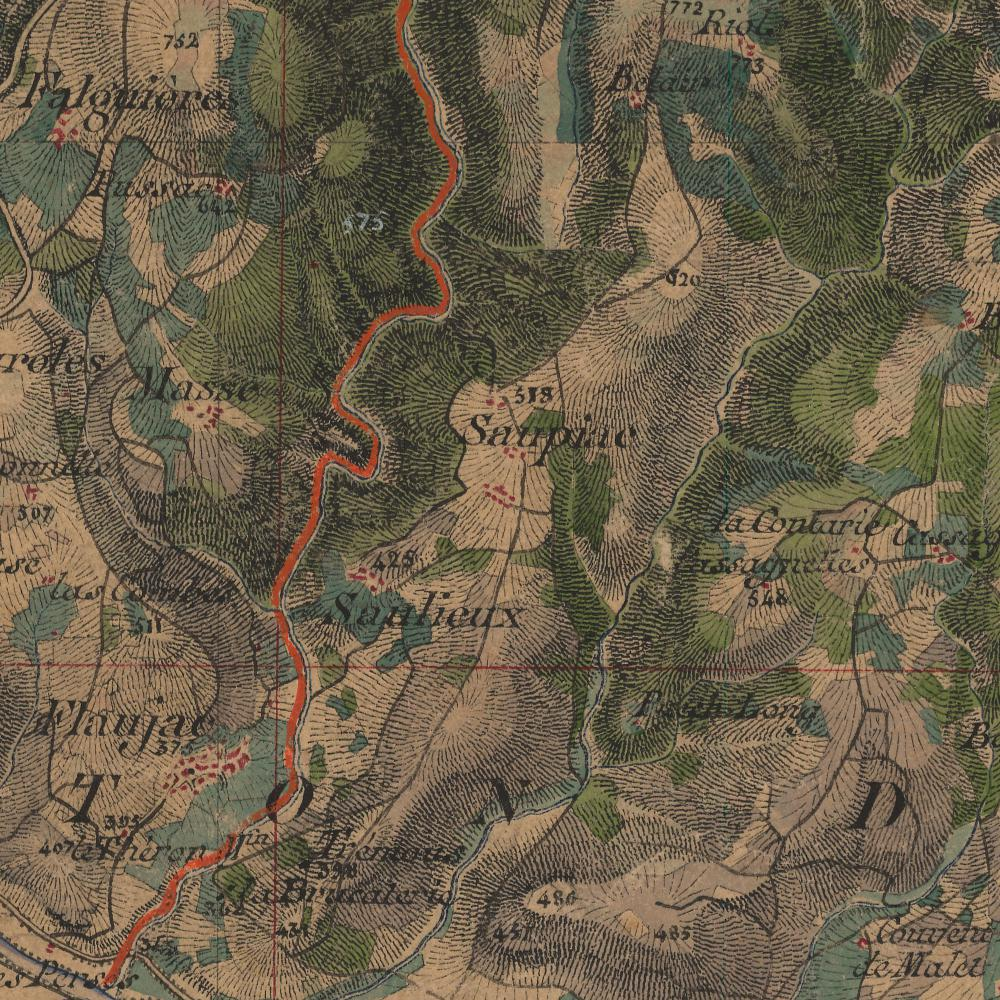
\includegraphics[width=0.5\textwidth]{figures/old_map.jpg}
\caption{\label{fig:org1afaa83}
Historical Maps}
\end{figure}

\section{Visualization of remote sensing data}
\label{sec:orged24fd1}
\subsection{Vizualization of remote sensing image}
\label{sec:org30da510}
The vizualisation  of remote  sensing images can  be done  either with
Monteverdi2  or QGIS\footnote{The  library \texttt{matplotlib}  of  python is  not
adapted to  visualize remote  sensing image  and should  be avoided.}.
QGIS might  be a  more efficient  when it  comes to  visualize several
images, or for the vizualisation of  vector layers. It will be used in
these labworks.

Most of  the information  regarding the  vizualisation of  raster data
with         QGIS         can          be         found         online
\url{http://docs.qgis.org/2.14/en/docs/user\_manual/working\_with\_raster/raster\_properties.html}.

More  generally,  to use  raster  data  with  QGIS is  described  here
\url{http://docs.qgis.org/2.14/en/docs/user\_manual/working\_with\_raster/index.html}.

In  this labwork,  a  few  properties will  be  reviewed  and you  are
encouraged to check (at least) the given references.

\subsubsection{Vizualization of grayscale image}
\label{sec:orgb073d70}
Open the image  \emph{fabas\_10\_12\_2013.tif} with QGIS. The default  view is a
colour composition, with the bands/channels association given in Table
\ref{tab:orgd3ceff1}. To start easy, we just open  one band at a time: right click
on  the  name  of  the  opened  image in  the  \emph{Layer}  pane  et  select
\emph{Properties}.   Then select  the tab  \emph{Style} and  \emph{Band rendering}.  In the
\emph{render type}, select \emph{Singleband gray} and the band you want to display.

You surely have to do \emph{Contrast enhancement}. Check the doc for that.

\begin{table}[htbp]
\caption{\label{tab:orgd3ceff1}
Bands and channels default association in QGIS (if there is not a set of specified spectral bands in the metadata).}
\centering
\begin{tabular}{rl}
\toprule
Band & Channel\\
\midrule
1 & Red\\
2 & Green\\
3 & Blue\\
\bottomrule
\end{tabular}
\end{table}

\begin{work}
\begin{enumerate}
\item Visualize  each  spectral  band  of the  data,  and  look  at  the
differences in terms of graylevel between spectral bands.
\item Zoom in/out: use the mousse's wheel to zoom into the image. What do
you observe ?
\end{enumerate}
\end{work}
\subsubsection{Vizualization of colour image}
\label{sec:org5cacd28}
Now you  can visualize  a colour images,  by selecting  three spectral
bands among those available  from the data. Again, \emph{Contrast
enhancement} should be done.

\begin{work}
\begin{enumerate}
\item Do a "true colours" and "false colours" compositions and compare what
is easily seen on each of them.
\item Get spectral  values for several pixels  corresponding to different
materials  (water,  grassland,  forest  and bare  soil). For that,
use the tool \emph{Identify features}, see
\url{http://docs.qgis.org/2.14/en/docs/user\_manual/introduction/general\_tools.html}
for detail.
\item Fill  the \emph{collaborative spreadsheet}  with your pixel values:
\begin{itemize}
\item \url{https://framacalc.org/fauvel\_rs\_water}
\item \url{https://framacalc.org/fauvel\_rs\_grassland}
\item \url{https://framacalc.org/fauvel\_rs\_forest}
\item \url{https://framacalc.org/fauvel\_rs\_baresoil}
\end{itemize}
\end{enumerate}
\end{work}
\subsection{Get data information}
\label{sec:orge532852}
Before  opening a  remote sensing  data, it  is possible  to get  some
information about its  properties. For instance, using  \texttt{gdalinfo} it is
possible to extract several information.  It can be used as

\begin{minted}[fontsize=\footnotesize,obeytabs=true,tabsize=4,bgcolor=bg]{sh}
gdalinfo fabas_10_12_2013.tif
\end{minted}

Help  on the function  can be obtained using  the command alone or by
doing :

\begin{minted}[fontsize=\footnotesize,obeytabs=true,tabsize=4,bgcolor=bg]{sh}
man gdalinfo
\end{minted}

Equivalently, it is possible to get the same information using the
function \texttt{otbcli\_ReadImageInfo} from the \emph{OTB-Applications}:

\begin{minted}[fontsize=\footnotesize,obeytabs=true,tabsize=4,bgcolor=bg]{sh}
otbcli_ReadImageInfo -in fabas_10_12_2013.tif
\end{minted}


\begin{work}
On the \emph{Fabas} data set, get the following information.
\begin{enumerate}
\item Number of lines, columns and bands,
\item Size of each pixel,
\item Numerical types for coding pixel values,
\item Position of the upper left pixel,
\item Projection.
\end{enumerate}
\end{work}
\section{Spectral indices: \emph{Normalized Difference Vegetation Index}}
\label{sec:org8402ba5}
Among the available  radiometric indices, only the  NDVI is considered
in this labwork. NDVI is widely used for vegetation monitoring because
it can be related to chlorophyll content and photosynthesis.

\begin{work}
\begin{enumerate}
\item Compute  the NDVI for each  \emph{Fabas} image.  You can  compute the NDVI
using several  ways, using  either \emph{OTB-Applications} or  the \emph{Raster
Calculator}
\url{http://docs.qgis.org/2.14/en/docs/user\_manual/working\_with\_raster/raster\_analysis.html\#raster-calculator}.
For a per  band analysis, both methods are  equivalent.  Using QGIS
provides the Graphical user interface,  which can be convenient for
processing  few images,  while  \emph{OTB-Applications}  allow to  process
large number of images using \emph{shell} programming.

Using the raster calculator, the following formula can be used (for
the Fabas image):

\begin{minted}[fontsize=\footnotesize,obeytabs=true,tabsize=4,bgcolor=bg]{sh}
   ("fabas_12_10_2013@4"-"fabas_12_10_2013@1")/("fabas_12_10_2013@4"+"fabas_12_10_2013@1")
\end{minted}

Using    the   \emph{OTB-Applications},    it   is    possible   to    use
\texttt{otbcli\_BandMath}. The syntax is similar, since we need to define the
image, the bands used and the expression of our processing:

\begin{minted}[fontsize=\footnotesize,obeytabs=true,tabsize=4,bgcolor=bg]{sh}
   otbcli_BandMath -il fabas_12_10_2013.tif -out ndvi_fabas.tif -exp "(im1b4-im1b1)/(im1b4+im1b1)"
\end{minted}

\item Compare the NDVI obtained for each date and explain your results.
\end{enumerate}
\end{work}
\section{Segmentation of remote sensing images}
\label{sec:org36458ef}
\subsection{Radiometric analysis}
\label{sec:org06831f9}
\begin{work}
For   the  \emph{near   infra  red}   band  and   the  NDVI   of  the   image
\textit{[2013-10-12 Sat]}, do
\begin{enumerate}
\item Look  at the  histogram and  identify the  local maxima.   For each
local  maximum, try  to identify  the corresponding  pixels in  the
image,
\item Keep track  of  the characteristics  of  each identified  maximum
(position and width).
\end{enumerate}
\end{work}
\subsection{Segmentation of 1D histogram}
\label{sec:org6bde535}
In  this part,  the  extraction  of image's  pixels  sharing the  same
\emph{radiometric behavior} is considered.  The  analysis of the histogram is
used to estimate this \emph{behavior}.   When only one material is segmented,
the output is a  binary image (image with value \texttt{0}  or \texttt{1}), where pixels
having  value \texttt{1}  are from  the same  material.  Figure  \ref{fig:orgb2704bf}
gives  an  example  of  such   outputs.   When  several  material  are
considered, the output is an images with integer values (\texttt{1}, \texttt{2}, \texttt{3} \ldots{}),
depending on the number of materials.

\begin{figure}[htbp]
\centering
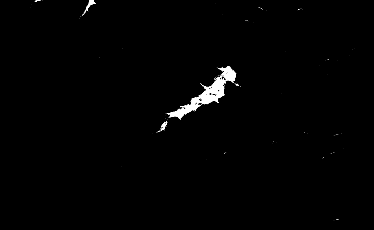
\includegraphics[width=0.65\linewidth]{./figures/quicklook_seg_eau.png}
\caption{\label{fig:orgb2704bf}
Binary image for Water.}
\end{figure}

A usual  work-flow is proposed  in this part.  First, QGIS is  used to
analyze the data and set-up the processing (parameters \emph{etc}). Then, the
\emph{OTB-Applications} are used to automatize the processing.

\begin{work}
For  the \emph{near  infra red}  band and  the NDVI,  segment the  identified
material. For  that, you need to  define interval of pixel  values for
which a  specific action  is done  (\emph{e.g.}, set  the value  to 0  or 1).
Implement the processing using the  \texttt{BandMath} application or the Raster
calculator.
\end{work}
\subsection{Graphical Modeler}
\label{sec:org1521c64}
For the segmentation of the NVDI, two processings are required
\begin{enumerate}
\item First, the computation of the NDVI from the original image,
\item Second,  the definition of  the interval  of values to  extract the
relevant pixels.
\end{enumerate}
With the graphical modeler, it is possible to define your workflow, to
automatize      complex      tasks.      Take      a      look      at
\url{http://docs.qgis.org/2.14/en/docs/user\_manual/processing/modeler.html}.  

\begin{work}
Define your model  to perform the segmentation of  intro three classes
of the NDVI.
\end{work}
\section{Change detection: \emph{Detection of floods}}
\label{sec:org6f3378f}
Change detection  in remote sensing consists  in detecting differences
between two  images, or  a set of  images.  It can  be used  to detect
changes in vegetation properties or in land cover.  It is also used in
disaster management, to detect impacted areas. In this labwork, we are
dealing with floods.  In Figure  \ref{org5ff5abe} is shown two quickbird images,
before  and  after a  flooding.   The  objective  is to  identify  the
impacted area to provide a map of these zones

\begin{figure}
\centering
\begin{tabular}{cc}
  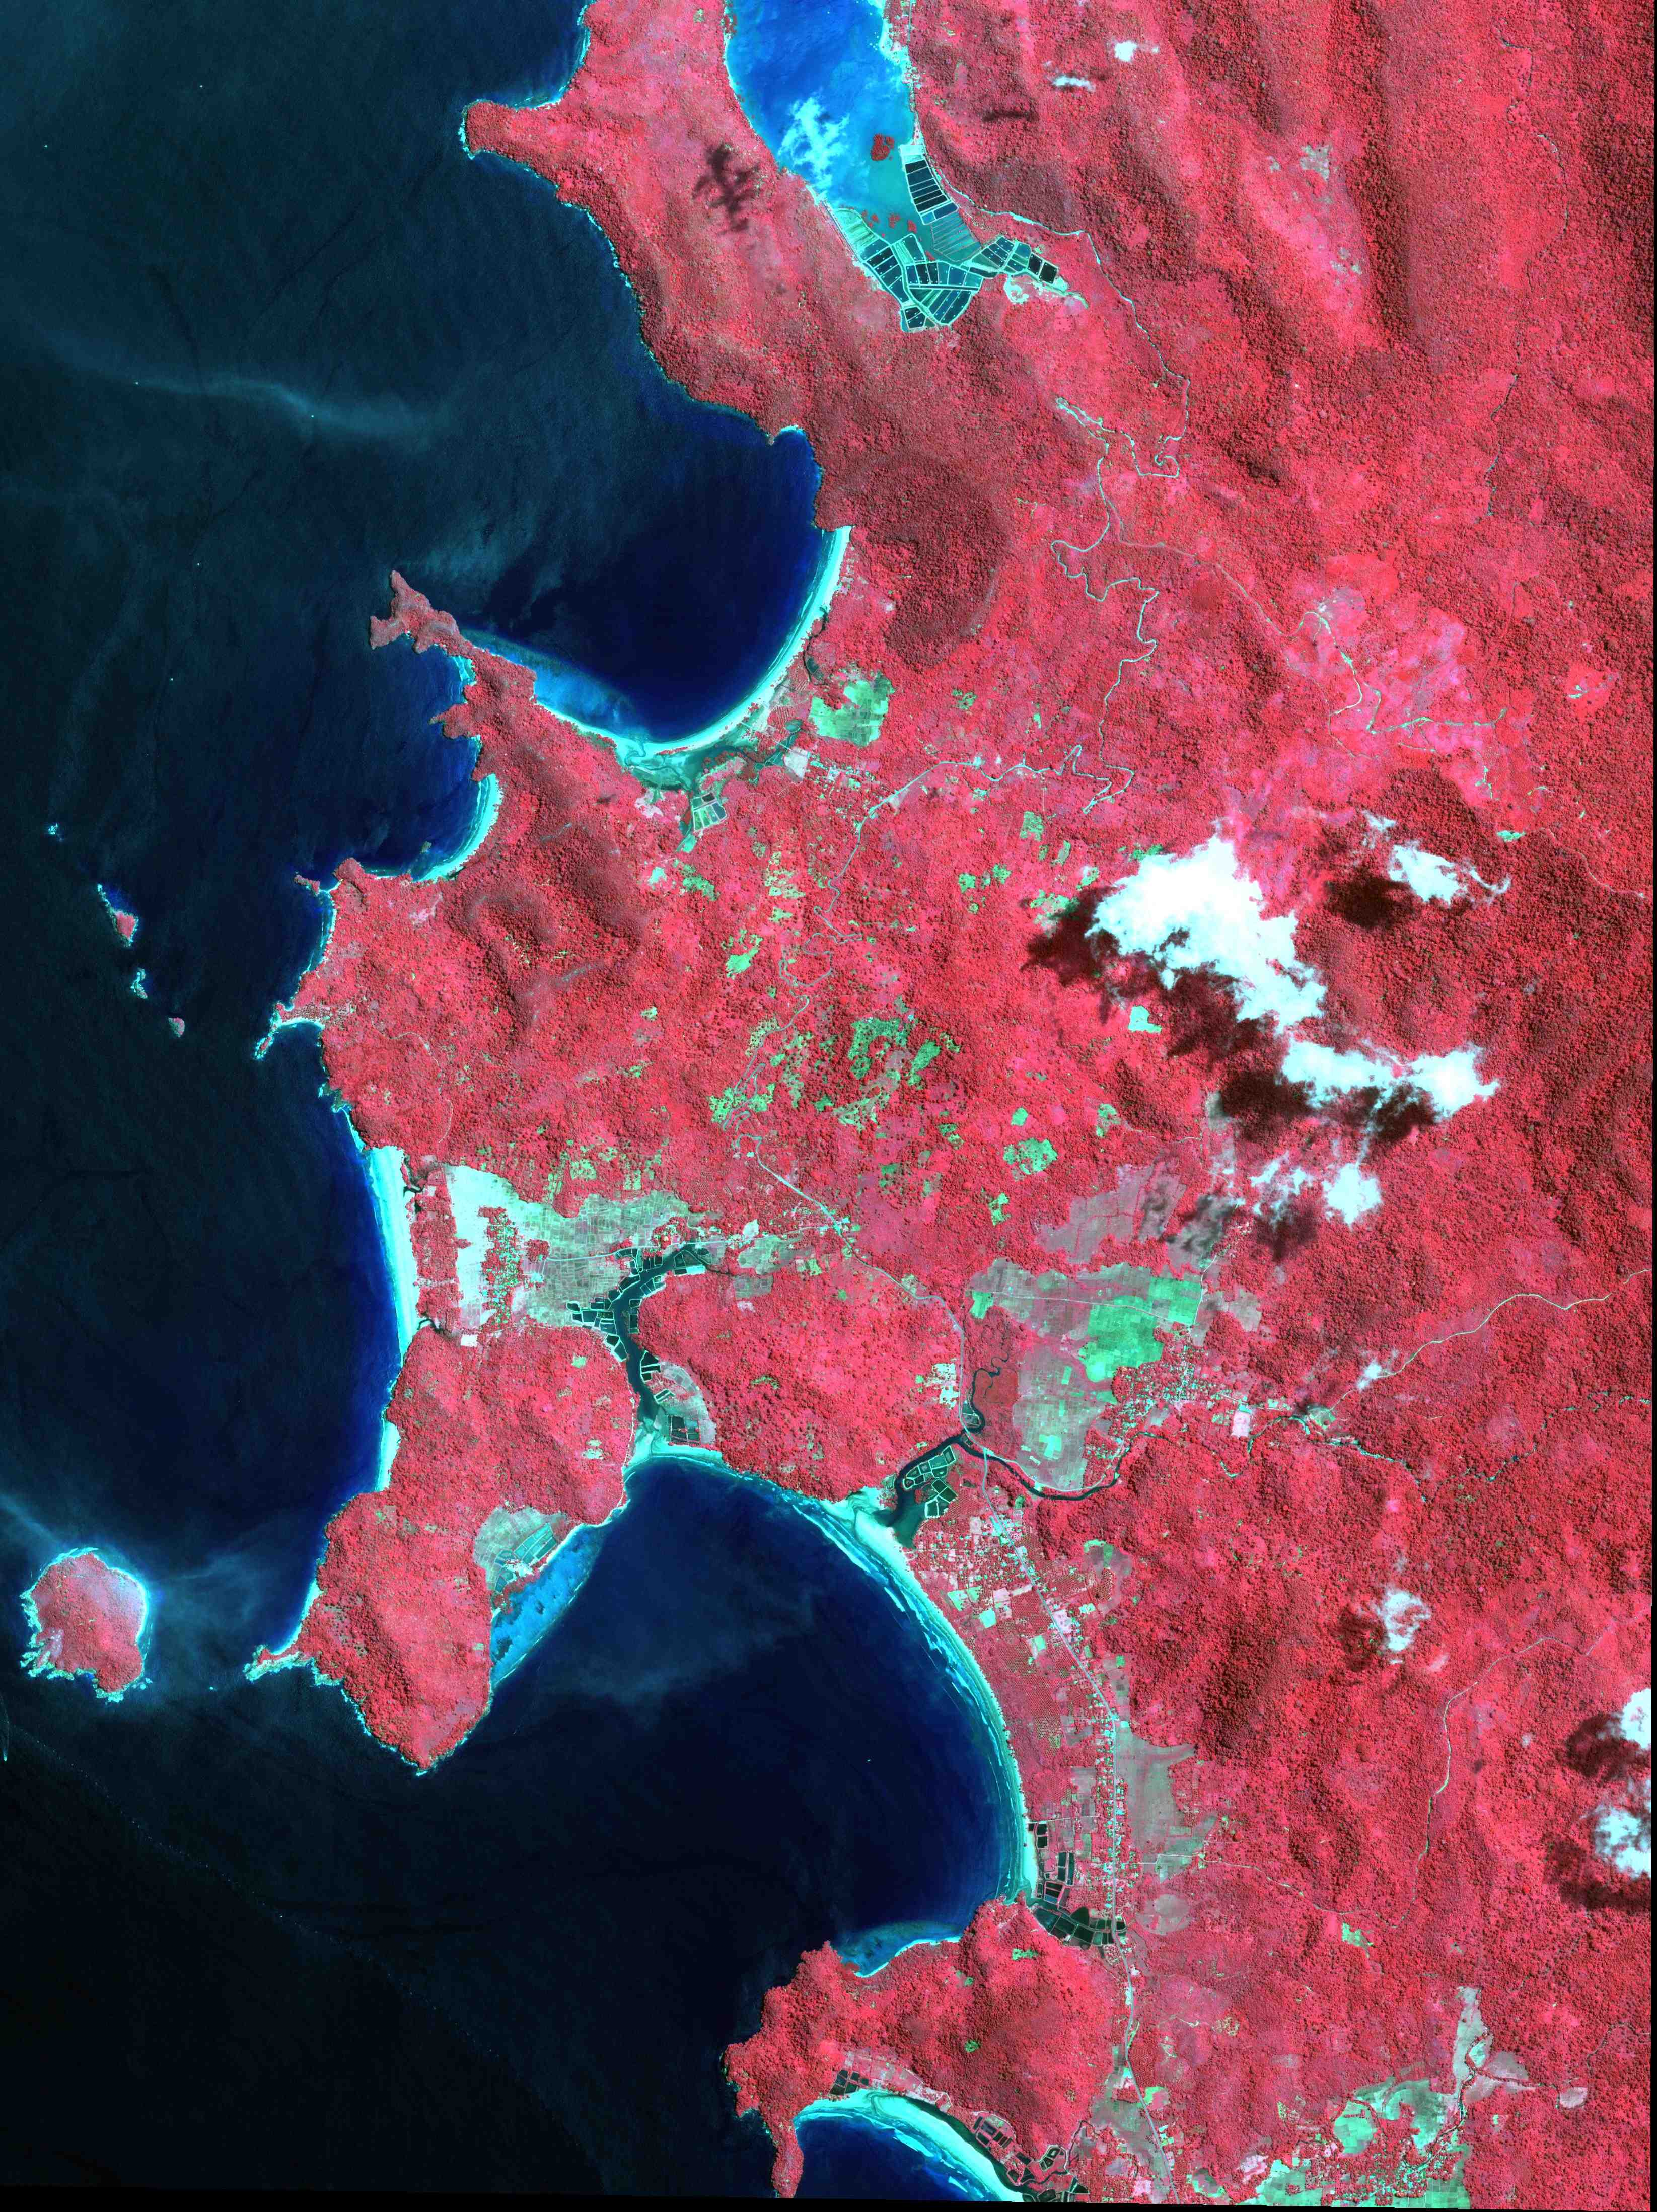
\includegraphics[width=0.45\linewidth]{figures/tsunami_before.jpg}&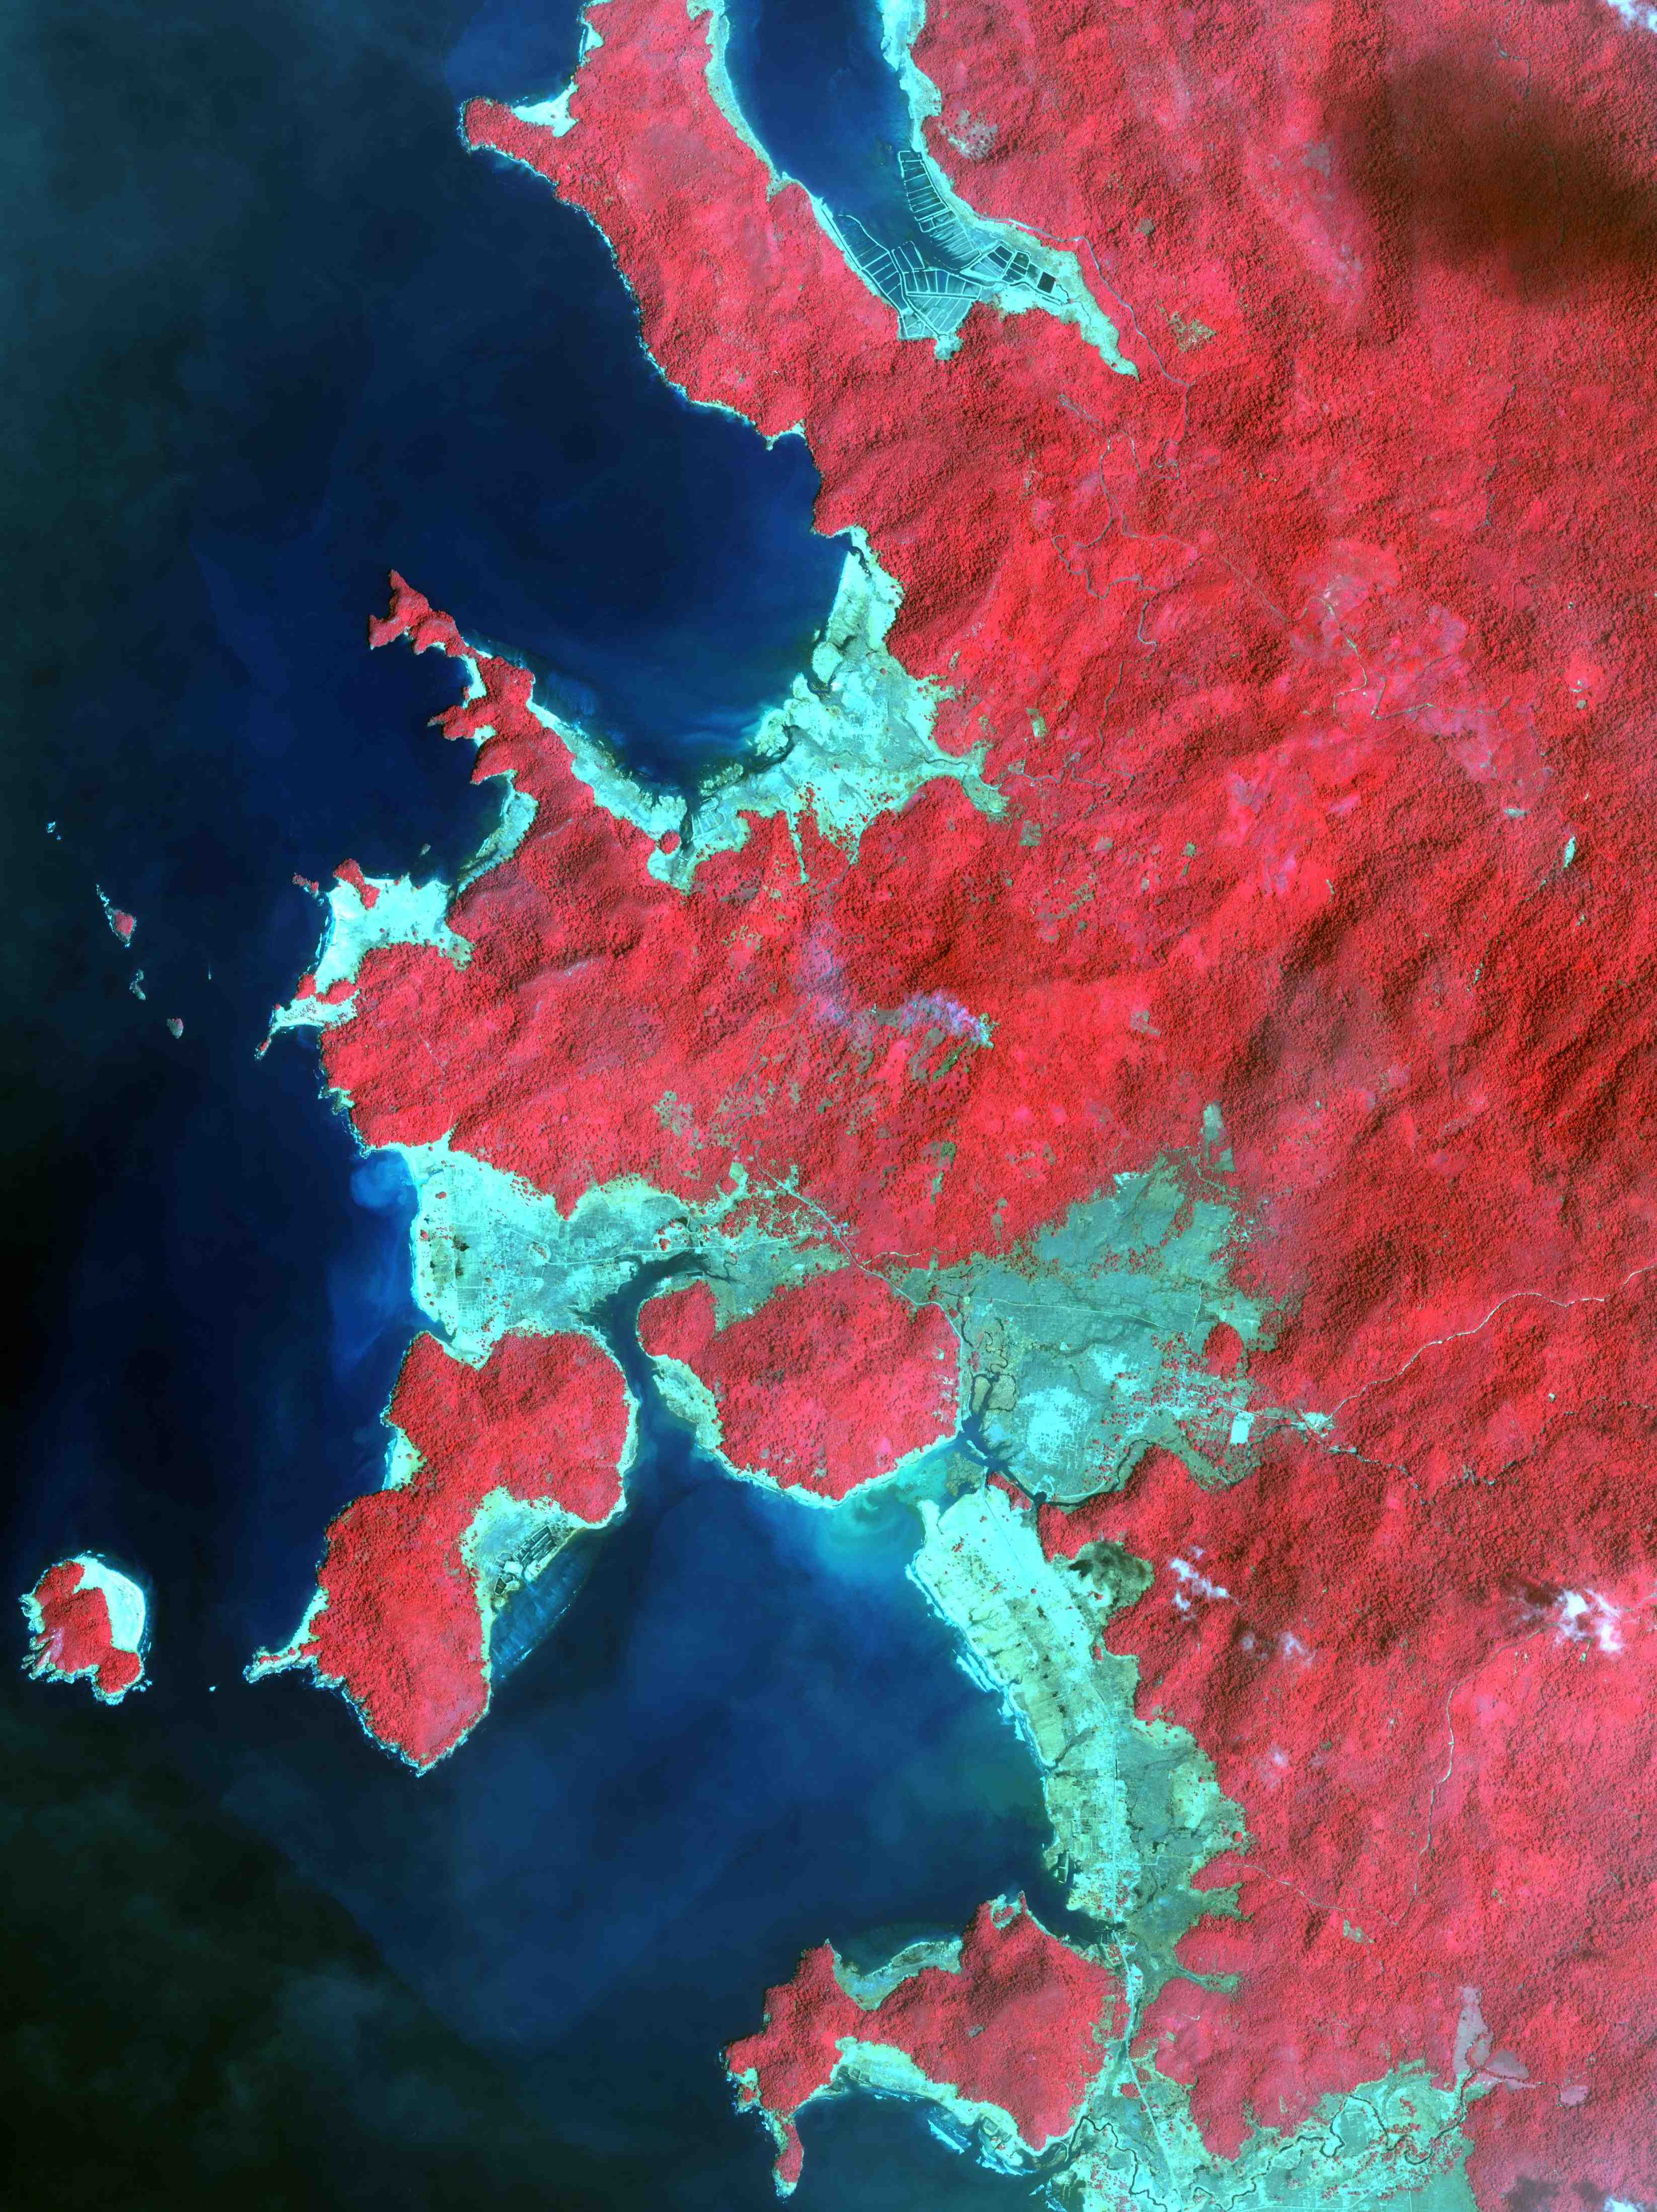
\includegraphics[width=0.45\linewidth]{figures/tsunami_after.jpg}\\
  (a)&(b)
\end{tabular}
\caption{\label{org5ff5abe}
False colours images of Lhonga Leupung area (a) before and (b) after flooding.}
\end{figure}

\begin{work}
\begin{enumerate}
\item Characterize the  impacted zones in terms  of radiometric behavior,
\emph{i.e.}, what is the variation in terms of spectral values. And why ?
\item Define the processing chain to extract these areas.
\item Implement the processing chain with the graphical modeler.
\item \uline{Optional}: Implement  the same processing chain  with shell scripts,
see \ref{sec:org89b1583}.
\end{enumerate}
\end{work}

\begin{figure}[htbp]
\centering
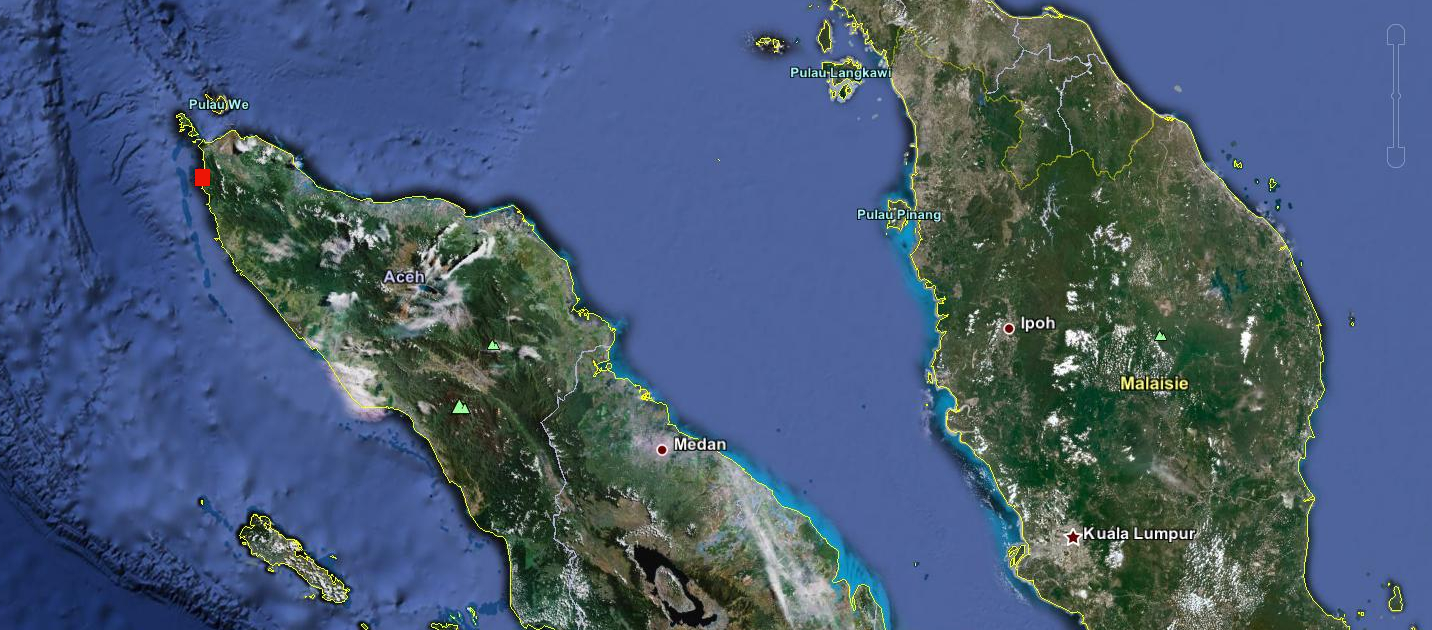
\includegraphics[width=0.75\textwidth]{./figures/google_bridge.jpg}
\caption{\label{fig:org7272ecb}
Google view of the impacted area. The red square represents the area of Figure \ref{org5ff5abe}.}
\end{figure}

\section{Classification of remote sensing images}
\label{sec:org37124d8}
\subsection{Introduction}
\label{sec:org4248364}
The aim  of this labwork  is to  perform the classification  of remote
sensing images using supervised algorithms.  The principle is the same
than segmentation.  But  now the gray level intervals  are not defined
manually and the  definition of a radiometric behavior  is not limited
to a rectangular area in  the spectral domain.  Furthermore, since all
the computation are  done by supervised algorithms, it  is possible to
use more information than one or  two bands and the full multispectral
image can be use.  In fact, more  than one image can be used.  In this
work, the  two \emph{Fabas} images  will be classified: first  separately and
then conjointly.

The  OTB  proposes  various  classifiers, each  one  having  different
characteristics.  In  order to train  (or learn) the  classifier, some
labeled pixels  should be  provided. It is  possible to  construct the
ground-truth (set of labeled pixels) in different ways:
\begin{itemize}
\item Using GIS layer and extract the relevant information at the pixel
level.
\item Do field survey and use GPS to identify pixels.
\item Do photo-interpretation when possible.
\end{itemize}
In this  works, the  ground-truth is  provided as  a vector  file, see
\ref{fig:org5da8560}.   Five  classes  are  considered,  they  are  given  in  Table
\ref{tab:org4b6f42a}.

\begin{figure}[htbp]
\centering
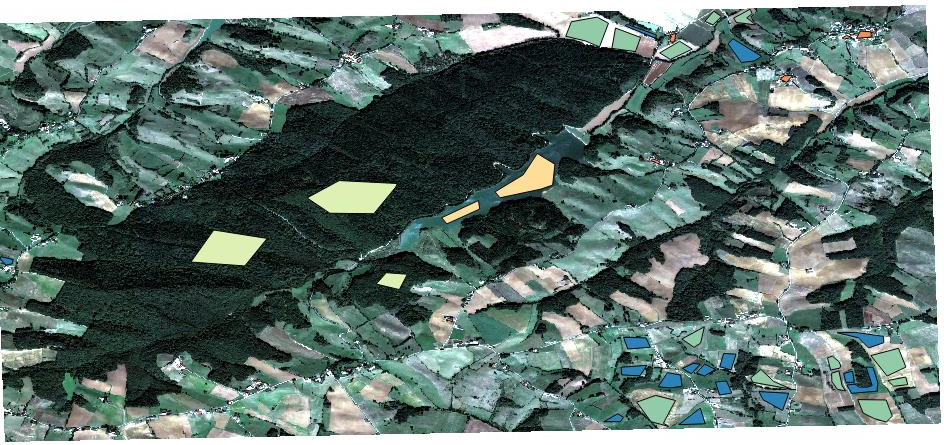
\includegraphics[width=0.75\textwidth]{./figures/label_fabas.jpg}
\caption{\label{fig:org5da8560}
Ground truth for the \emph{Fabas} image.}
\end{figure}

\begin{table}[htbp]
\caption{\label{tab:org4b6f42a}
Classes of interest. Numbers corresponding to the attribute in the GIS file is also given.}
\centering
\begin{tabular}{cccccc}
\toprule
\textbf{Classes} & Sparse vegetation & Bare soil & Woody vegetation & Water & Built up\\
\midrule
\textbf{Attribute} & 1 & 2 & 3 & 4 & 5\\
\bottomrule
\end{tabular}
\end{table}

During  this  labwork,   it  is  proposed  to  compare   in  terms  of
classification accuracy  and processing  time some of  the classifiers
proposed in OTB and all the combination of input data, \emph{i.e.}:
\begin{itemize}
\item K-nn, Bayes, SVM and Random Forest.
\item The ground-truth  being composed  of pixels from  one date,  and two
\emph{concatenated} dates.
\end{itemize}
\subsection{Getting started with OTB}
\label{sec:orgabcf6a1}
There are several steps to do a classification.
\begin{enumerate}
\item \emph{Learn   the    classifier}:   It    is   done    with
\texttt{TrainImagesClassifier}.   It takes  as inputs,  the (set  of) remote
sensing  image(s), the  ground-truth (in  vector format),  and some
parameters of the method.  To learn the classifier, only the pixels
inside the  ground-truth are  used. After this  step, a  \emph{model} that
contains the parameters  is saved. If asked, a  confusion matrix is
computed.
\item \emph{Classify the image}: Once the  classifier is learned, it is possible
to apply the model to all the  pixels of the image.  It can be done
with \texttt{ImageClassifier}.
\item Compute the  accuracy of  the  thematic map  according to  some
groundthruth. \textbf{This groundthruth should  not be spatially correlated
with  the one  used  for  training}.  The  confusion  matrix can  be
computed using the function \texttt{ComputeConfusionMatrix}.
\end{enumerate}


\begin{work}
This should be done for one image and one classifier only.
\begin{enumerate}
\item Learn the model,
\item Apply the model to classify the entire image,
\item Compute the confusion matrix and save it in a \emph{csv} file.
\item Open  the CSV  using a spreadsheet.   From the  confusion matrix,
compute the following indices:
\begin{itemize}
\item Global accuracy,
\item Producer accuracy,
\item User accuracy.
\end{itemize}
\end{enumerate}
\end{work}

\subsection{Automatize the process with scripts (shell or python)}
\label{sec:orgf9b97fb}
It  is possible  to run  directly  the \emph{OTB-Applications}  from the  the
command line  (on linux-based  OS). This  way, it  is possible  to run
several  operations  on   one  data  set  or  on   several  data  sets
automatically.  A brief introduction to command line tools is given in
Appendix \ref{sec:org89b1583}.

The  three previous  \emph{OTB-Applications} are  available from  the command
line interface (CLI), same name with the prefix \texttt{otbcli\_} :

\begin{itemize}
\item \texttt{otbcli\_TrainImagesClassifier},
\item \texttt{otbcli\_ImageClassifier},
\item \texttt{otbcli\_ComputeConfusionMatrix}.
\end{itemize}

The same  inputs than in  QGIS should  be provided (\emph{raster  and vector
file},  \emph{algorithm parameters  \ldots{}}). For  instance,  if you  are in  the
directory where the data are, learning the KNN classifier with default
parameters do the following, classifying the whole image and computing
the confusion matrix reduce to

\begin{minted}[fontsize=\footnotesize,obeytabs=true,tabsize=4,bgcolor=bg]{sh}
otbcli_TrainImagesClassifier \
    -io.il fabas_12_10_2013.tif \
    -io.vd train_fabas.shp \
    -classifier knn \
    -io.out model.mod
otbcli_ImageClassifier \
    -in fabas_12_10_2013.tif \
    -model model.mod \
    -out fabas_classif.tif
otbcli_ComputeConfusionMatrix \
    -in fabas_classif.tif \
    -out matconf.csv \
    -ref vector \
    -ref.vector.in valid_fabas.shp
\end{minted}

This is nothing else than what you provide in QGIS ! In the following,
we are  going to combine  Python scripts  and the OTB  Applications to
define our  processing chain. Two python  modules will be use:  \href{https://docs.python.org/2/library/os.html}{os} and
\href{https://docs.python.org/2/library/glob.html}{glob}.  These modules  are very convenient to manage  files, folder and
to launch applications. Also, we are going to benefit Python abilities
to process strings.

Let's start with an example, to run the first application

\begin{minted}[fontsize=\footnotesize,obeytabs=true,tabsize=4,bgcolor=bg]{python}
# Load the module
import os

# Launch the application
os.system('otbcli_TrainImagesClassifier -io.il fabas_12_10_2013.tif -io.vd train_fabas.shp -classifier knn -io.out model.mod')
os.system('otbcli_ImageClassifier -in fabas_12_10_2013.tif -model model.mod -out fabas_classif.tif')
os.system('otbcli_ComputeConfusionMatrix -in fabas_classif.tif -out matconf.csv -ref vector -ref.vector.in valid_fabas.shp')
\end{minted}

or equivalently:

\begin{minted}[fontsize=\footnotesize,obeytabs=true,tabsize=4,bgcolor=bg]{python}
# Load the module
import os

# Define processing
train = 'otbcli_TrainImagesClassifier -io.il fabas_12_10_2013.tif -io.vd train_fabas.shp -classifier knn -io.out model.mod' 
classify = 'otbcli_ImageClassifier -in fabas_12_10_2013.tif -model model.mod -out fabas_classif.tif'
validate = 'otbcli_ComputeConfusionMatrix -in fabas_classif.tif -out matconf.csv -ref vector -ref.vector.in valid_fabas.shp'

# Launch the application
os.system(train)
os.system(classify)
os.system(validate)
\end{minted}

Additional usefull references are  given section \ref{sec:orge34ee6c}, take the
time to read them.

\begin{work}
\begin{enumerate}
\item Write  the script  to learn  the model  for all  the classification
methods and with each date.  Each time extract the confusion matrix
and compute the global accuracy and the class average accuracy.
\item Report the results on the \emph{collaborative spreadsheet}: \url{https://framacalc.org/fauvel\_res\_classification}
\item For  the best method  in terms of classification  accuracy, discuss
about the errors obtained with the confusion matrix.
\item Classify the  whole image  and  compare by  visual inspection  the
errors with what you have inferred from the confusion matrix.
\end{enumerate}
\end{work}
\subsection{Influence of the spatial distribution of the learning samples}
\label{sec:orgc61cfcd}
In order to evaluate the influence of the validation samples, you will
investigate  several   reference  layers  to  compute   the  confusion
matrix. Since OTB only select a few samples from all the available one
(can be  controlled with  the options  \texttt{samples.mt} and  \texttt{samples.mv}), we
need to repeat the experiment several times, to avoid bias.

\emph{Select one classifier  for all the experiments. You  are encouraged to
define a python script.}

\begin{work}
Repeat \uline{20} times the following test:
\begin{enumerate}
\item Learn with \emph{train\_fabas} and compute the confusion matrix with
\emph{train\_fabas}. Save the confusion matrix for each repetition.
\item Learn  with  \emph{train\_fabas}  and compute  the  confusion  matrix  with
\emph{valid\_fabas}. Save the confusion matrix for each repetition.
\item Compute the average global accuracy and the mean class accuracy and
their standard deviation. \emph{You can check the figure \ref{org9d8debc} to do it automatically}.
\end{enumerate}


Discuss about the results. 
\end{work}

\begin{figure}
\begin{minted}[fontsize=\footnotesize,obeytabs=true,tabsize=4,bgcolor=bg]{python}
import scipy as sp
import glob
# get all the csv files that match the pattern and order the list in increasing order
NAMES_TRAIN,NAMES_VALID = glob.glob('confu_train_*.csv'),glob.glob('confu_valid_*.csv')
NAMES_TRAIN.sort()
NAMES_VALID.sort()

oa_train,oa_valid = [],[]

for name_train,name_valid in zip(NAMES_TRAIN,NAMES_VALID):
    temp = sp.genfromtxt(name_train,delimiter=',',skip_header=2) # read the file, skeap the two first lines (of comments)
    oa = 100*sp.diag(temp).sum()/temp.sum() # Compute the overall accuracy
    oa_train.append(oa) # add the values to the list
    temp = sp.genfromtxt(name_valid,delimiter=',',skip_header=2)
    oa = 100*sp.diag(temp).sum()/temp.sum()
    oa_valid.append(oa)
    
# Compute mean accuracy and standard deviation and save the results
res = [[sp.mean(oa_train),sp.std(oa_train)],[sp.mean(oa_valid),sp.std(oa_valid)]]
sp.savetxt('acc.csv',res,delimiter=',',fmt='%1.3f')
\end{minted}
\caption{\label{org9d8debc}
Sample code to process a set of \texttt{csv} files.}
\end{figure}
\section{Satellite Image Time Series}
\label{sec:org9092424}
\subsection{Objectives}
\label{sec:org573ef1b}
The objectives  of this part are  two-folds. First, it is  proposed to
build  a Satellite  Image Time  Series (SITS)  given a  set of  images
acquired  over  the  same  area.   Then,  we  are  going  to  classify
winter/summer crops  using the SITS. Reference  and validation samples
were extracted from the \href{https://www.data.gouv.fr/fr/datasets/registre-parcellaire-graphique-2012-contours-des-ilots-culturaux-et-leur-groupe-de-cultures-majorita/}{RPG} for  the same year. Table \ref{tab:org3c50403} provides
the different classes available of  these area. Details about the data
are given \ref{sec:orgdbb25a6}.

\begin{table}[htbp]
\caption{\label{tab:org3c50403}
RPG nomenclature and conversion used in the labwork}
\centering
\begin{tabular}{rllr}
\toprule
Value & Label & Class & Attribute\\
\midrule
1 & Wheat & Winter Crop & 1\\
2 & Grain maize and silage & Summer Crop & 2\\
3 & Barley & Winter Crop & 1\\
4 & Other cereals & Winter Crop & 1\\
5 & Rapeseed & Winter Crop & 1\\
6 & Sunflower & Summer Crop & 2\\
7 & Other oleaginous & Summer Crop & 2\\
8 & Protein crops & Summer Crop & 2\\
15 & Grain leguminous & Winter Crop & 2\\
16 & Fodder & Grassland & 3\\
18 & Permanent grassland & Grassland & 3\\
19 & Temporary meadows & Grassland & 3\\
\bottomrule
\end{tabular}
\end{table}

\subsection{Construction of the SITS}
\label{sec:orgbfa3b31}
Before classifying the  SITS, you need to built it.  In these labwork,
two SITS  will be considered. One  build will all the  spectral bands,
and the other one using the NDVI only.

\begin{work}
\begin{enumerate}
\item Compute the NDVI for each date,
\item Concatenate all the dates,
\begin{itemize}
\item For  the spectral bands  (\emph{i.e.} all the  blue bands, then  all the
green bands \ldots{}),
\item For the NDVI
\end{itemize}
\item Using QGIS,  plot the  temporal  profile for  several objects  and
discuss of their shape w.r.t the phenology.
\end{enumerate}
\end{work}
\subsection{Classification of the SITS}
\label{sec:orgee1e637}
Two scenario will be considered in this labwork. Classification of the
whole SITS and classification of the \emph{best date.}

\begin{work}
\emph{With the classifier of your choice}
\begin{enumerate}
\item Do the classification of the  whole SITS given the training layers,
and compute the predicted thematic map, restricted to pixels inside
the RPG  (use the  mask provided). Compute  classification accuracy
using  the  validation   layer  and  report  the   results  in  the
\emph{collaborative spreadsheet}.
\item Do the  classification for  each date  independently, compute  the
classification accuracy and report the results in the \emph{collaborative
spreadsheet}. \emph{Tips: It can (must) be automatized \ldots{}}
\end{enumerate}
\end{work}
\subsection{Extraction of the best couple of dates}
\label{sec:orga06ec28}
We have seen in the previous part that one date is not enough to get a
correct classification rate. In that section, we are going to test all
the  possible couple  of  dates, to  find  the best  one  in terms  of
classification accuracy. 

How to do it ? Just test  all the possible combinations! Be aware that
using \texttt{t1}  and \texttt{t2} is  the same than  using \texttt{t2} and  \texttt{t1}. Here we  have 13
dates, so the  total number of couples is  . I really
hope you can use bash script now \ldots{}

The code given  figure \ref{orgf019799} might help you.  It extracts all
the  possible  couples  of files  from  a  set  of  files in  a  given
directory, the files ended with \texttt{*m.tif}.

\begin{figure}
\begin{minted}[fontsize=\footnotesize,obeytabs=true,tabsize=4,bgcolor=bg]{sh}
FILE=`ls *m.tif` # Get all the files that end with 'm.tif'
EFILE=''
for file in $FILE
do
    # Add  variables to  be excluded  from the  second loop:  EFILE ->
    # Exclude file
    EFILE=`echo $EFILE $file`

    # Exclude these variables from the next loop
    FILES=$FILE # Copy the variable
    for efile in $EFILE
    do
	FILES=`echo  $FILES |  sed "s/\b$efile\b//g"`  # Exclude  from
						    # FILES   all  the
						    # file  from EFILE
						    # (substitute with
						    # nothing)
    done

    # Do the process, given the couple of images
    for files in $FILES
    do
	echo Process file $file and $files
	# Add  you  code here  to  process  the data:  concatentation,
	# training and extraction of the confusion matrix
	echo ${file:17:8}${files:17:8} #  Name of the input  data : to
				       # be  use to  set  name of  the
				       # confusion matrix
    done
    echo ""
done
\end{minted}
\caption{\label{orgf019799}
Bash script to get all the possible couples of files.}
\end{figure}
Analyze the three best results in terms of accuracy. Interpret the
results given the classes to be classified, the geographical area and
its practical consideration (should we buy the complete SITS, or just
some periods of the years? \ldots{})
\section{Dynamic Habitat Index}
\label{sec:org1835e2c}
\subsection{Introduction}
\label{sec:org76a166d}
In this labworks, we are going to compute several indices of habitat
dynamic's in order to define several ecozones. It is bases on the
following paper: 

\begin{quote}
Nicholas C. Coops, Michael A. Wulder, Dennis C. Duro, Tian Han, Sandra
Berry,  The development  of  a Canadian  dynamic  habitat index  using
multi-temporal  satellite   estimates  of  canopy   light  absorbance,
Ecological  Indicators,  Volume  8,  Issue 5,  September  2008,  Pages
754-766,                        ISSN                        1470-160X,
\url{http://dx.doi.org/10.1016/j.ecolind.2008.01.007}.
(\url{http://www.sciencedirect.com/science/article/pii/S1470160X08000071})
\end{quote}

These indicators underly vegetation dynamic, they are usually computed
in the \emph{fraction of photosynthetically active radiation (fPAR)} absorbed
by the vegetation.  However these data  are not available.  So in this
lab, the NDVI will be used. The data is described in \ref{sec:orgdbb25a6}.


\begin{work}
The first (easy)  part is to convert NDVI values  to fPAR like values.
Since fPAR is a fraction, its values  are between 0 and 1. You have to
convert the interval  range of NDVI to  0 and 1 using  a simple linear
function: \(f(x)=ax+b\). You have to find \(a\) and \(b\) !
\begin{eqnarray*}
  f:[-1,1] &\to& [0,1]\\
  x&\mapsto&f(x)=ax+b
\end{eqnarray*}
\end{work}

\subsection{Construction of the SITS}
\label{sec:org0291a11}
Before analyzing the  SITS, you need to built it.   
\begin{work}
\begin{enumerate}
\item Compute the NDVI for each date,
\item Convert to fPAR-like values,
\item Concatenate all the dates,
\item Using QGIS,  plot the  temporal  profile for  several objects.
\end{enumerate}
\end{work}

\subsection{Computation of the dynamic indices}
\label{sec:orgda96baa}
The second part of the labwork  concern the computation of the dynamic
indices.   Let  us  note  the  vector   of  fPAR  values  of  pixel  i
\(\mathbf{x}_i=[\mathbf{x}_i(t_1),\ldots,\mathbf{x}_i(t_d)]\).     Three
indices have been defined:
\begin{enumerate}
\item The cumulative annual greenness,
\end{enumerate}
$$CG = \sum_{j=1}^d\mathbf{x}_i(t_j)$$
\begin{enumerate}
\item The annual minimum cover,
\end{enumerate}
$$MC = \min_{j}\left[\mathbf{x}_i(t_1),\ldots,\mathbf{x}_i(t_j),\ldots,\mathbf{x}_i(t_d)\right]$$
\begin{enumerate}
\item The greenness coefficient of variation.
\end{enumerate}
$$GCV = \frac{\sigma_{\mathbf{x}_i}}{\mu_{\mathbf{x}_i}}$$

\begin{work}
\begin{enumerate}
\item Write the python scripts to compute all indices.
\item Concatenate all the indices into one multiband image.
\end{enumerate}
\end{work}
\subsection{Characterization of ecozones}
\label{sec:org95e2fe3}

Perform a  segmentation of the SITS  using the three indices  as input
values. A  primarily study suggests  the number  of ecozones is  \texttt{4} for
this area. Look at the function \texttt{otbcli\_KMeansClassification} to perform
the automatic segmentation of you data.

\begin{work}
\begin{enumerate}
\item Performs the segmentation with 4 classes and save the values of the
estimated centroid.
\item Extract the values of the centroid and interpret their values in
terms of habitat.
\item Do a visual validation of your results on the thematic map.
\end{enumerate}
\end{work}
\section{Appendix}
\label{sec:org2fa86d7}
\subsection{Short introduction to shell}
\label{sec:org89b1583}
This section provides  an introduction to \emph{shell}  programming and \emph{shell
scripts}.   A script  is a  set of  commands, which  allows to  write a
processing chain  for a given image,  or to apply one  processing to a
set  of   images.   Of   course,  mixing   these  two   situations  is
possible. You  can find  more information  easily on  the web,  a good
starting point can be the \href{https://en.wikibooks.org/wiki/Bash\_Shell\_Scripting}{Wikibook}.

Shell is  a programming  language that is  available on  all GNU/Linux
distributions. It  can be used  directly from the  prompt (interactive
mode), or  by writing a file  with a set  of commands to be  run. This
file should start with the line

\begin{minted}[fontsize=\footnotesize,obeytabs=true,tabsize=4,bgcolor=bg]{sh}
#!/bin/bash
\end{minted}
In  the following,  it is  assumed  that we  are working  on the  file
\texttt{script.sh}. To insert comment inside the script, the symbol \texttt{\#} has to be
used.

\begin{minted}[fontsize=\footnotesize,obeytabs=true,tabsize=4,bgcolor=bg]{sh}
# This is a comment
\end{minted}
With Linux, a file can be  \emph{writable}, \emph{readable} and/or \emph{executable}. To be
run as a script, it should be at least \emph{executable} by the OS. It can be
by done by running the following command:

\begin{minted}[fontsize=\footnotesize,obeytabs=true,tabsize=4,bgcolor=bg]{sh}
chmod +x script.sh
\end{minted}
To run it, just do

\begin{minted}[fontsize=\footnotesize,obeytabs=true,tabsize=4,bgcolor=bg]{sh}
./script.sh
\end{minted}

\subsubsection{Basic commands}
\label{sec:org8005f13}
\begin{itemize}
\item \textbf{cd}: Change directory. To enter a directory, do \texttt{cd Name\_Of\_Directory}.
\item \textbf{ls}: List all the file in the current directory.
\item \textbf{pwd}: Return the name of the current directory.
\item \textbf{cp}: Copy a file/directory, for instance \texttt{cp A B}.
\item \textbf{mv}: Move a file to another, for instance \texttt{mv A B}.
\item \textbf{mkdir}: Create a directory, \texttt{mkdir Name\_Of\_Directory}.
\end{itemize}

For instance, to get all the \texttt{tif} files in the current folder:

\begin{minted}[fontsize=\footnotesize,obeytabs=true,tabsize=4,bgcolor=bg]{sh}
ls *tif
fabas_10_12_2013.tif  fabas_12_10_2013.tif
\end{minted}

\subsubsection{Variables}
\label{sec:org2edae10}
In shell, a variable is a string (not a number). It can be defined as:

\begin{minted}[fontsize=\footnotesize,obeytabs=true,tabsize=4,bgcolor=bg]{sh}
var1='Mathieu' # Store "Mathieu" in variables "var1"
var2='Fauvel'
var3='34'
\end{minted}

Be  careful to  spaces: there  are no  spaces, otherwise  an error  is
returned!  A  variable is  displayed using the  \texttt{echo} function  and the
variable is accessed with the command \texttt{\$}.

\begin{minted}[fontsize=\footnotesize,obeytabs=true,tabsize=4,bgcolor=bg]{sh}
echo $var1 $var2      # print "Mathieu Fauvel"
echo "$var3 ans"      # print "33 ans"
echo '$var3 ans'      # print "$var3 ans"
\end{minted}

\begin{minted}[fontsize=\footnotesize,obeytabs=true,tabsize=4,bgcolor=bg]{sh}
Mathieu Fauvel
34 ans
$var3 ans
\end{minted}

Note the  difference between the simple  quote \texttt{'} and the  double quote
\texttt{"}. The  simple quote does not  evaluate the variable while  the double
quote does.

It is possible to pass parameters to the script, solely by adding them
when the  script is called.  They are  accessible using the  command \texttt{\$}
following by the order number of appearance when the script is
called. Let define the \texttt{script.sh} file.

\begin{minted}[fontsize=\footnotesize,obeytabs=true,tabsize=4,bgcolor=bg]{sh}
# ./script.sh Name FamilyName Age
echo $1 $2
echo "J ai (eu) $3 ans !"
\end{minted}

When we do this, we have the following output:

\begin{minted}[fontsize=\footnotesize,obeytabs=true,tabsize=4,bgcolor=bg]{sh}
chmod +x script.sh
./script.sh Mathieu Fauvel 33
\end{minted}

\begin{minted}[fontsize=\footnotesize,obeytabs=true,tabsize=4,bgcolor=bg]{sh}
Mathieu Fauvel
J ai (eu) 33 ans !
\end{minted}

\subsubsection{Loop}
\label{sec:org6d79cec}
As in any programming language, loop are very useful to apply a series
of processing  to several  elements of a  sequence. The  example below
applies a processing on all \emph{tif} files of the current directory:

\begin{minted}[fontsize=\footnotesize,obeytabs=true,tabsize=4,bgcolor=bg]{sh}
for i in *.tif # For all tif file
do
    cp $i ndvi_$i # create a new file and add ndvi_ at the beginning of the filename
done
\end{minted}
\subsubsection{Sequence}
\label{sec:org7fe2694}
It is possible to define sequences of string like this:

\begin{minted}[fontsize=\footnotesize,obeytabs=true,tabsize=4,bgcolor=bg]{sh}
for name in bayes libsvm knn rf
do
    echo $name
done
\end{minted}

\begin{minted}[fontsize=\footnotesize,obeytabs=true,tabsize=4,bgcolor=bg]{sh}
bayes
libsvm
knn
rf
\end{minted}

Sequences of numbers can be defined like this:

\begin{minted}[fontsize=\footnotesize,obeytabs=true,tabsize=4,bgcolor=bg]{sh}
for i in `seq 1 5`
do
echo $i
done
\end{minted}

\begin{minted}[fontsize=\footnotesize,obeytabs=true,tabsize=4,bgcolor=bg]{sh}
1
2
3
4
5
\end{minted}
\subsection{Short introduction to Python}
\label{sec:orge34ee6c}
A     good    starting     point     is     the    following     link:
\url{http://kitchingroup.cheme.cmu.edu/pycse/pycse.html}.   Here,   I   just
review few things that are usefull  for the labwork. But python is far
more than this short introduction.
\subsubsection{String}
\label{sec:org37908c5}
Handling  strings with  python is  very easy.  It is  possible to  add
strings together, as with number! Pay attention to spaces\ldots{}

\begin{minted}[fontsize=\footnotesize,obeytabs=true,tabsize=4,bgcolor=bg]{python}
name="Mathieu"
surname="Fauvel"
print name + surname
\end{minted}

\begin{verbatim}
MathieuFauvel
\end{verbatim}

To use numbers in strings, it is necessary to convert them, using the function \texttt{str}

\begin{minted}[fontsize=\footnotesize,obeytabs=true,tabsize=4,bgcolor=bg]{python}
print "Bonjour j\'ai eu " + str(33) + " ans"
\end{minted}

\begin{verbatim}
Bonjour j'ai eu 33 ans
\end{verbatim}

\subsubsection{Loop}
\label{sec:orgb114d54}
It is very  easy to iterate over  a list with python. The  list can be
made of numbers, strings etc \ldots{}  Since a list is \href{https://docs.python.org/2/glossary.html}{iterable}, defining a
\texttt{for} loop is just:

\begin{minted}[fontsize=\footnotesize,obeytabs=true,tabsize=4,bgcolor=bg]{python}
listeNumber = [1,2,3,4]
print listeNumber
for item in listeNumber:
    print(item)

listeString = ['knn','bayes','libsvm','rf']
print listeString
for item in listeString:
    print(item)
\end{minted}

\begin{verbatim}
[1, 2, 3, 4]
1
2
3
4
['knn', 'bayes', 'libsvm', 'rf']
knn
bayes
libsvm
rf
\end{verbatim}

\subsubsection{Glob}
\label{sec:org2c9bf62}
The \href{https://docs.python.org/2/library/glob.html}{glob} module finds all the  path-names matching a given pattern. It
uses standard Unix (shell) path  expansion rules. However, results are
returned in arbitrary order and therefore sometimes ordering operation
is necessary. It returns a list  of pathnames, or a iterator which can
be useful  for large  processing. Below  some examples  to see  how it
works. First, check what is in my \emph{figures} directory:

\begin{minted}[fontsize=\footnotesize,obeytabs=true,tabsize=4,bgcolor=bg]{sh}
ls figures/
\end{minted}

\begin{verbatim}
google_bridge.jpg
label_fabas.jpg
label_fabas.jpgw
old_map.jgw
old_map.jpg
pixel.pdf
quicklook_fabas_10_12_2013.jpg
quicklook_fabas_12_10_2013.jpg
quicklook_seg_eau.png
sits_f2.pgw
sits_f2.png
take5spot5.png
tsunami_after.jpg
tsunami_before.jpg
\end{verbatim}

If we want to get all the files, we just need to do

\begin{minted}[fontsize=\footnotesize,obeytabs=true,tabsize=4,bgcolor=bg]{python}
import glob

files = glob.glob("figures/*")
for files_ in files:
    print files_
\end{minted}

\begin{verbatim}
figures/sits_f2.png
figures/quicklook_fabas_12_10_2013.jpg
figures/tsunami_after.jpg
figures/take5spot5.png
figures/sits_f2.pgw
figures/quicklook_fabas_10_12_2013.jpg
figures/pixel.pdf
figures/label_fabas.jpg
figures/tsunami_before.jpg
figures/old_map.jpg
figures/quicklook_seg_eau.png
figures/label_fabas.jpgw
figures/old_map.jgw
figures/google_bridge.jpg
\end{verbatim}

If we only want the \emph{png} files:

\begin{minted}[fontsize=\footnotesize,obeytabs=true,tabsize=4,bgcolor=bg]{python}
import glob

files = glob.glob("figures/*.png")
for files_ in files:
    print files_
\end{minted}

\begin{verbatim}
figures/sits_f2.png
figures/take5spot5.png
figures/quicklook_seg_eau.png
\end{verbatim}

The iterator is \texttt{iglob}, it does the same job than \texttt{glob}, but without storing all the results simultaneously.

\begin{minted}[fontsize=\footnotesize,obeytabs=true,tabsize=4,bgcolor=bg]{python}
import glob

for files_ in glob.iglob("figures/*.png"):
    print files_
\end{minted}

\begin{verbatim}
figures/sits_f2.png
figures/take5spot5.png
figures/quicklook_seg_eau.png
\end{verbatim}

\subsubsection{Argparse}
\label{sec:org699e82a}
Argparse (\url{https://docs.python.org/3.6/library/argparse.html}) is module
to parse  options and  arguments from  the command-line  interface. It
defines what  are the  mandatory argument,  generates help  and usages
messages and errors at runtime. 

For instance,  suppose we have  a function that needs  two parameters:
the  name  of a  multispectral  file  and  the  size of  the  template
filter. Argparse handles everything:

\begin{minted}[fontsize=\footnotesize,obeytabs=true,tabsize=4,bgcolor=bg]{python}
import argparse

# Initialization of the filter
parser = argparse.ArgumentParser()

# Add arguments
parser.add_argument("-in",dest="image",help="Image to be processed",type=str)
parser.add_argument("-p",help="Size of the template",type=int,default=1)

args = parser.parse_args()

print args.image
print args.p
\end{minted}

\begin{verbatim}
None
1
\end{verbatim}
\end{document}